%!TEX output_directory = ./tmp/

\documentclass[11pt]{article}

\usepackage{amsmath}
\usepackage{amsfonts}
\usepackage{textcomp}
\usepackage{graphicx}
\usepackage{graphics}

\usepackage{caption}
\usepackage{subfig}

\usepackage{float}

\usepackage[top=0.8in, bottom=0.8in, left=0.8in, right=0.8in]{geometry}
% Add other packages here %
\usepackage{xcolor}
\usepackage{color}
\definecolor{bg}{RGB}{235,235,235}
\newcommand{\java}[1]{\colorbox{bg}{\textcolor{red}{\usefont{OT1}{cmtt}{m}{n}#1}}}


% Put your group number and names in the author field %
\title{\bf Exercise 2: A Reactive Agent for the Pickup and Delivery Problem}
\author{Group \textnumero: 15 - Hadrien Hendrikx, Yuxiang Li}

% the report should not be longer than 3 pages

\begin{document}
\maketitle

\section{Problem Representation}

\subsection{Representation Description}
% describe how you design the state representation, the possible actions, the reward table and the probability transition table

Our reactive agent is based on Markov Decision Process. We define $\mathcal{C} = \{1 .. N\}$ the set of cities and $\mathcal{A} = \{P, M\}$ the set of actions: pickup and move. In our case, a \textbf{state} $s \in \mathcal{C}^2$ is uniquely defined by the source city $c_{src}$ and the destination of the package $c_{pkg}$ (if there is no package, the package destination is set to the source city itself). An \textbf{action} $a \in \mathcal{A} \times \mathcal{C}$ is defined by a type of action $t$ associated with a destination $c_{dest}$. 

In addition to states and actions, we note $d(c_{src},c_{dest})$ the distance, or cost, between 2 cities $c_{src}$ and $c_{dest}$. Then $r(c_{src},c_{pkg})$ refers to the income of carrying the package from $c_{src}$ to $c_{pkg}$ and finally $p(c_{src},c_{pkg})$ the probability of having a package from city $c_{src}$ to $c_{pkg}$. Under these notations, \textbf{reward table} $R$ and \textbf{transition table} $T$ are defined as follow:

\begin{align*}
  R \colon \mathcal{C}^2 \times \mathcal{A} \times \mathcal{C} &\to \mathbb{R} \\
  (c_{src}, c_{pkg}, t, c_{dest}) &\mapsto 
  \begin{cases} 
	  r(c_{src},c_{pkg}) - d(c_{src},c_{dest}), & \mbox{if } t = P \\ 
	  - d(c_{src},c_{dest}), & \mbox{if } t = M 
  \end{cases} 
\end{align*}

\begin{align*}
  T \colon \mathcal{C}^2 \times \mathcal{A} \times \mathcal{C} \times \mathcal{C}^2 &\to [0, 1] \\
  (c_{src}, c_{pkg}, t, c_{dest}, c_{src}', c_{pkg}') &\mapsto 
  \begin{cases} 
	  p(c_{src}',c_{pkg}'), & \mbox{if } t = P \mbox{ and } c_{pkg} = c_{dest} = c_{src}' \\ 
	  p(c_{src}',c_{pkg}'), & \mbox{if } t = M \mbox{ and } c_{dest} = c_{src}' \\ 
	  0, & \mbox{otherwise} 
  \end{cases} 
\end{align*}

\subsection{Implementation Details}
% describe the implementation details of the representations above and the implementation details of the reinforcement learning algorithm you implemented

\subsubsection{New classes for state and action}

We create 2 new classes: \java{State} for states and \java{MDPAction} for actions. \java{State} contains the source city $c_{src}$, the package destination $c_{pkg}$ and a list of possible actions. Given one state, the possible actions are: 1) pick up a package and go to the destination; 2) decline (if there is) a package and move to a neighboring city. \java{MDPAction} is even simpler, it contains the type of action $t$ and the destination $c_{dest}$. There exists an injection from \java{MDPAction} to \java{Action} provided by Logist package so we can translate our action descriptor to real action in the simulation. It should also be noticed that the hash value of those objects is calculated using the city's ID, the type of action and the maximum ID value to avoid any duplicates. We are going to use them in the lookup tables.

\subsubsection{Lookup table}

The quickest way to build a lookup table is to use a N-dimensional array whose index is based on ID value. However, this makes the code difficult to read as the dimension of our input is large. Instead of using ID, we use hashable objects, \java{State} and \java{MDPAction}, as index of our lookup tables, e.g. $Q(s,a)$, $V(s)$ and policy $\pi(s)$.  Here is the signature of our lookup tables:

\begin{itemize}
	\item $Q$ table: \java{Map<City, Map<MDPAction, Double>>}
	\item $V$ table: \java{Map<State, Double>}
	\item Policy $\pi$ table: \java{Map<State, MDPAction>}
\end{itemize}

We use a map of map to handle 2 inputs in the $Q$ table.

\subsubsection{Reachable states}

As we can see from the definition of transition table, each state has a small number of reachable states that we can pre-compute. In our implementation, we compute this list of reachable states for every state, which accelerates the evaluation of the expected future value.

\subsubsection{Learning steps}

We fix the learning steps to 1,000 at maximum, but a lower value is also sufficient if the discount factor is not very big. There are 2 conditions to terminate the learning process: 1) enough learning steps; 2) the improvement of $Q$ is less than $10^{-6}$. 

\section{Results}
% in this section, you describe several results from the experiments with your reactive agent

\subsection{Experiment 1: Discount factor}
% the purpose of this experiment is to understand how the discount factor influences the result

\subsubsection{Setting}
% you describe how you perform the experiment (you also need to specify the configuration used for the experiment)

We compare 5 agents with different discount factors: 0, 0.25, 0.5, 0.75 and 1. All agents begin with Paris.

\subsubsection{Observations}
% you describe the experimental results and the conclusions you inferred from these results
From figure 1, we can make 2 observations:

\begin{itemize}
	\item The average reward converges faster with small discount factor
	\item Larger discount factor leads to bigger reward (except when the factor is equal to 1)
\end{itemize}

A small discount factor gives more importance to imminent rewards in which case the agent usually has a short-term plan. A short-term plan allows the agent to increase his profit quickly, which explains why average reward converges faster (a, b and c from Figure 1). However, this strategy ignores the possibility of getting bigger reward in the long term. When the number of steps is larger, the average reward is higher when the discount factor is big (a and c from Figure 1). Meanwhile, the case where the discount factor equals to 1 is an exception as there is no convergence of the policy, which leads to worse result (c and d from Figure 1). 

\subsection{Experiment 2: Comparisons with dummy agents}
% you compare the results of your agent with two dummy agents: the random agent that was already given in the starter files and another dummy agent that you define and create. You should report the results from the simulations using the topologies given in the starter files and optionally, additional topologies that you create.

\subsubsection{Setting}
% you describe how you perform the experiment and you describe the dummy agent you created (you also need to specify the configuration used for the experiment)

In addition to the random agent, we introduce the \textit{greedy agent}. The greedy agent knows his current average reward. When a new task appears, he evaluates his new average reward if he picks up the package. If the new reward is bigger, he picks up, otherwise he moves to a random neighboring city. We compare these 2 dummy agents with reactive agents used in previous experiment (France, start with Paris).

\subsubsection{Observations}
% elaborate on the observed results

On Figure 1, we notice that reactive agents, no matter how larger the discount factor is, are better than the random agent with a pickup rate of 0.85. Meanwhile, our greedy agent is almost as good as reactive agents. At least, it achieves a similar result compared to the reactive agent with a discount factor of 0. In addition, the greedy agent progresses faster at the beginning.

At the end of simulation, the reactive agent with a discount factor of 0.75 performs 1.3 times better than the random agent and 1.05 times better than the greedy agent.

\begin{figure}
\centering
\subfloat[Reactive, Discount 0.0]{
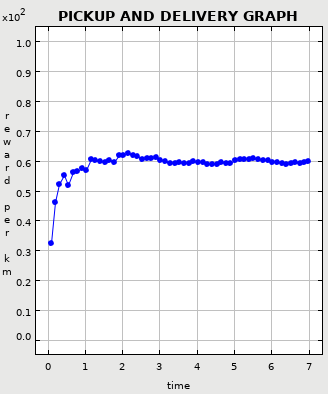
\includegraphics[width=0.3\textwidth]{img/000.png}
}\hfill
\subfloat[Reactive, Discount 0.25]{
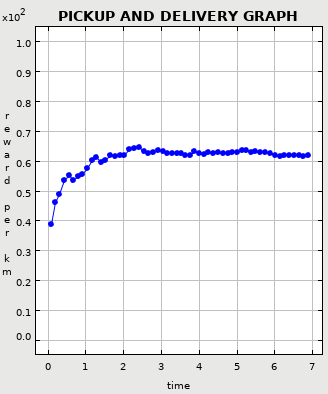
\includegraphics[width=0.3\textwidth]{img/025.png}
}\hfill
\subfloat[Reactive, Discount 0.75]{
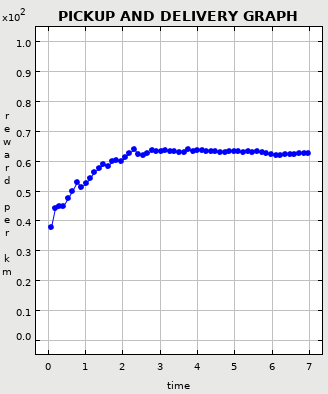
\includegraphics[width=0.3\textwidth]{img/075.png}
}

\subfloat[Reactive, Discount 1.0]{
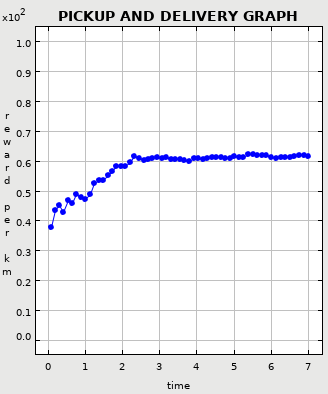
\includegraphics[width=0.3\textwidth]{img/100.png}
}\hfill
\subfloat[Random, Pickup rate 0.85]{
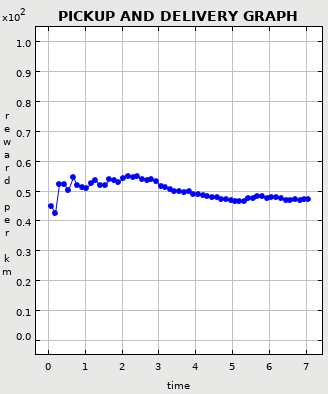
\includegraphics[width=0.3\textwidth]{img/rand.png}
}\hfill
\subfloat[Greedy]{
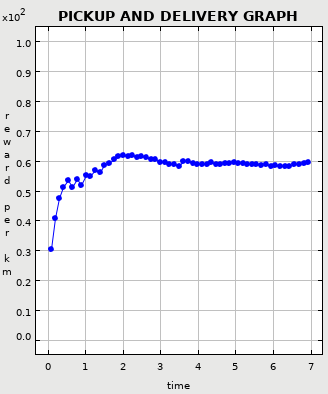
\includegraphics[width=0.3\textwidth]{img/lazy.png}
}

\caption{Results of simulation}
\end{figure}

\end{document}